\documentclass[12pt]{article}
\usepackage[a4paper,
left=15mm,
right=15mm,
top=20mm,
bottom=20mm]{geometry}
\usepackage{amsmath}
\usepackage{graphicx}
\usepackage{algorithm}
\usepackage{algorithmic}
\usepackage{multicol}
\usepackage{amsthm}
\usepackage{bm}
\usepackage{fancyhdr}
\usepackage{amssymb}
\usepackage{sidecap}
\usepackage{hyperref}
\usepackage{titlesec}
\usepackage{array}


\newcolumntype{P}[1]{>{\centering\arraybackslash}p{#1}}  %per centrare le colonne nelle tabelle
\newcolumntype{M}[1]{>{\centering\arraybackslash}m{#1}} %per centrare le righe nelle tabelle
\renewcommand{\arraystretch}{1.5} %per spaziare le righe in una tabella

\newcommand\tab[1][1cm]{\hspace*{#1}}
\renewcommand{\labelitemii}{$\star$}



\titleformat*{\subsubsection}{\large\bfseries}


\begin{document}


\begin{titlepage}
	\begin{center}
		\vspace*{1cm}
		
		\Huge
		\textbf{FastGAN: Faster and Stabilized GAN}
		\vspace{1.5cm}
		
		\Large
		Authors:\\
		\textbf{Mauro Ficorella 1941639}\\
		\textbf{Martina Turbessi 1944497}\\
		\textbf{Valentina Sisti 1952657}\\
		\vspace{0.5cm}
		
		\vfill
		
		
\includegraphics[width=0.4\textwidth]{Images/Logo.jpg}
		
		\vfill
		
		\vspace{0.8cm}
		
		\Large
		Sapienza\\
		May 2021
	\end{center}
\end{titlepage}


\newpage
\pagestyle{fancy}
\fancyhf{}
\fancyfoot[R]{\thepage}
\rhead{Mauro Ficorella, Martina Turbessi, Valentina Sisti}
\lhead{FastGAN}

% ABSTRACT --------------------------------------------------------------------

\begin{center}
	
	\normalsize\MakeUppercase{\textbf{Abstract}\vspace*{0.35cm}}
	
	\begin{minipage}[t]{0.6\textwidth}
	\textit{The main aim of FastGAN is to allow users with limited computing budget and resources to 
	train a GAN. Moreover it eliminates the requirement of a big dataset for training.
	These are big advantages since traditional GANs required a lot of GPU computational power
	(i.e. one or more server-level GPUs with at least 16 GB of VRAM in StyleGAN2) and a large number of 
	images for training. 
	This implementation allowed to train from scratch on a NVIDIA GeForce RTX 2070 SUPER and a 
	NVIDIA GeForce GTX 1050-Ti, obtaining good results also on a small dataset. 
	The structure of FastGAN comprehends a Skip-Layer channel-wise Excitation (SLE) module and a self-supervised
	Discriminator trained as a feature-encoder.\\
	This GAN outperforms StyleGAN2 and other traditional GANs in terms of computational requirements
	and training time.
	}
	\end{minipage}

\end{center}

\vspace*{1cm}
% INTRODUCTION --------------------------------------------------------------------
\section{Introduction}
\large
State-of-the-art (SOTA) GANs, despite having a lot of usage (implications) in real life applications, 
such as photo editing, diseases diagnosis, image translation and artistic creation, their high cost in 
terms of computational power and dataset size made their usage very limited in contexts with a very small
computational budget. More specifically, there are three main problems afflicting GANs' training:
\begin{itemize}
	\setlength\itemsep{0.01em}
	\item \textit{Accelerate training}: this problem has been approached from various perspectives, but this brought
			only very limited improvements in training speed, while not enhancing quality within the shortened training time;
	\item \textit{High resolution training}: this made GAN much harder to converge, since the increased model parameters
			lead to a more rigid gradient flow to optimize $G$, and since the target distribution made by images at high resolution
			is super sparse. There was some approaches trying to solve this problem, but they led to a slightly greater computational
			cost, consuming more GPU memory and requiring more training time;
	\item \textit{Stabilize training}: mode-collapse on generator $G$ is a big challenge when training GANs, given fewer training
			samples and lower computational power and budgets (smaller batch-size). $D$ is unable to provide consistent gradients to 
			train $G$, since is more likely to be overfitting on the datasets. There were, also here, approaches that tryed to solve this 
			problem, but they have limited using scenarios and image domain, and worked only on low resolution images with unlimited computing
			resources.
\end{itemize}
\begin{figure}[H]
	\centering
	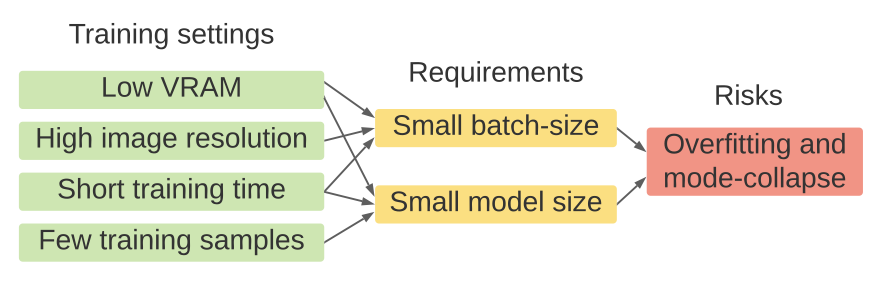
\includegraphics[width=0.5\textwidth]{Images/problems.png}
	\caption{FastGAN training challenges.} 
\end{figure}
In some situations a possible way to avoid these problems was the \textit{transfer-learning} using pre-trained models,
but this solution had the disadvantage of the lack of guarantee to find dataset compatible with the pre-training. 
Another way was \textit{fine-tuning}, but this gave even worse results in terms of performance.
Those approaches were not took in consideration by people who wanted to train their model from scratch, in order to 
avoid biases typic of the fine-tuned pre-trained models; in other cases there were the necessity to train models
with datasets containing less than 100 images.
A possible workaround for the situation of a small dataset was \textit{dynamic data-augmentation}, but the cost of SOTA models
remained very high.\\\\
This paper aims to learn an unconditional GAN requiring, at the same time, low computational power and small datasets
for training. In order to do this, FastGAN has a ``fast-learning" generator $G$ and a discriminator $D$ able to continuously
return signals very useful to train $G$. FastGAN reaches the above objectives based on the following two techniques:
\begin{itemize}
	\setlength\itemsep{0.01em}
	\item \textbf{Skip-Layer channel-wise Excitation module}: revises channel responses on high-scale feature-maps using
			low-scale activations and allows to reach a faster training using a more robust gradient flow throughout the 
			model weights;
	\item \textbf{Self-supervised discriminator $D$ trained as a feature-encoder with an extra decoder}: this discriminator
			is forced to learn a feature-map that covers more regions from an image in input; in this way it gives richer
			signals in order to train $G$. It has been shown that \textit{auto-encoding} is the best self-supervision strategy for $D$.
\end{itemize} 

% METHOD -------------------------------------------------------------------------

\section{Method}
\large	

\begin{figure}[H]
	\label{fig:fig2}
	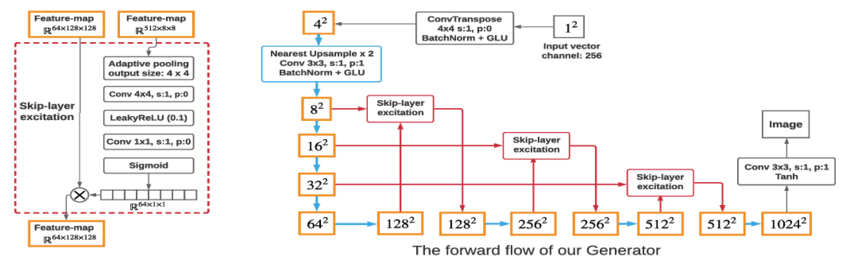
\includegraphics[width=1\textwidth]{Images/structure.png}
	\caption{
		On the left is represented the structure of the skip-layer excitation,
		on the right is represented the structure of the generator $G$. 
		Feature-maps are the yellow boxes, up-sampling structures are represented 
		by blue boxes and blue arrows, SLE modules are the red boxes.
		}
\end{figure}
In order to optimize GANs with respect to the SOTA models, in FastGAN is adopted a lightweight model, 
using a single convolutional layer on each resolution in the generator $G$; moreover, on the high resolutions
in both generator $G$ and discriminator $D$, only three channels for the convolutional layers are applied in 
input and output. As said before this structure helps making FastGAN faster to train, remaining, at the same time,
strong on small datasets. 

\subsection{Skip-Layer Channel-Wise Excitation}

In the traditional GANs the generator $G$ required more convolutional layers (and so a deeper model) to synthesize 
high resolution images, and this led to longer training times. 
In order to train such a deep model it was used the Residual structure (ResBlock), increasing the computational cost.
Traditionally ResBlock implements the skip-connection as an element-wise addition between the activations from different
convolutional layers, but with the requirement that the spatial dimensions of the activations are the same.
Moreover, previously, skip-connections were only used within the same resolution.\\\\
FastGAN, instead, uses a different approach through the two following strategies:
\begin{itemize}
	\setlength\itemsep{0.01em}
	\item {	
	In order to eliminate the complex computation of convolution, it is used multiplication between activations, instead of 
	addition, giving to one side of activations the spatial dimension of $1^2$.
	}
	\item {
	Instead of performing skip-connection only within the same resolution, here it is performed between resolutions with a much
	longer range ($8^2$ and $128^2$, $16^2$ and $256^2$, $32^2$ and $512^2$); this follows from the fact that an equal spatial-dimension
	is no longer required.
	}
\end{itemize} 
Using the above techniques, SLE keeps the advantages of ResBlock with a shortcut gradient flow, while not requiring an extra computation
load.\\\\
The Skip-Layer Excitation module is defined as:
\begin{equation}
	\mathbf{y} = \mathcal{F}(\mathbf{x}_{low}, \{\mathbf{W}_i\})\cdot \mathbf{x}_{high}
\end{equation}
In function $\mathcal{F}$ there are the operations on $\mathbf{x}_{low}$; module weights to be learned 
are represented by $\mathbf{W}_i$; $\mathbf{x}$ is the input feature-map of the SLE module, while $\mathbf{y}$
is its output feature-map. As shown in the \hyperref[fig:fig2]{Figure 2}, the SLE module is composed by the 
feature-map $\mathbf{x}_{low}$ at resolution $8 \times 8$ and the feature-map $\mathbf{x}_{high}$ at resolution $128 \times 128$.\\
First of all, $\mathcal{F}$ contains an adaptive average-pooling layer that down-samples $\mathbf{x}_{low}$ into $4 \times 4$; then
there is the convolutional-layer that further down-samples it into $1 \times 1$. Moreover non-linearity is modeled by a \textit{LeakyReLU},
and after that another convolutional-layer is used to let $\mathbf{x}_{low}$ having the same channel size as $\mathbf{x}_{high}$. 
Finally there is a \textit{Sigmoid} function that does a gating operation, and then the output from $\mathcal{F}$ is multiplied with 
$\mathbf{x}_{high}$ along the channel dimension, returning $\mathbf{y}$ with the same shape as $\mathbf{x}_{high}$.\\\\
The above Skip-Layer Excitation works between feature-maps that are far away from each other, brings the benefit of the channel-wise
feature re-calibration and makes the whole model’s gradient flow stronger; moreover it enables the generator $G$ to automatically 
disentangle the content and style attributes. It has also be shown that, starting from another synthesized sample, and replacing 
$\mathbf{x}_{low}$ in the Skip-Layer Excitation, the generator $G$ can generate an image in the same style of the new replacing 
image and with the content unchanged. 

\subsection{Self-Supervised Discriminator}

\begin{figure}[H]
	\label{fig:fig3}
	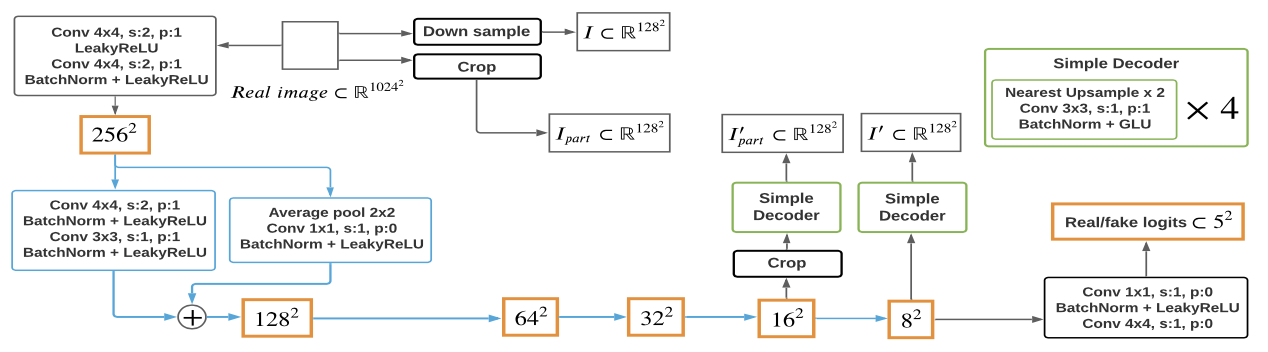
\includegraphics[width=1\textwidth]{Images/discriminator.png}
	\caption{
		Here is represented the structure and the forward flow of the discriminator.
		The same residual down-sampling structure is represented by the blue boxes and blue arrows,
		the same decoder structure is represented by the green boxes.
		}
\end{figure}

The discriminator $D$ is handled as an encoder and trained using small decoders. In this way the decoders can give good reconstructions
of the images thanks to the image features that the decoder $D$ is forced to extract. Moreover a simple reconstruction loss, which is 
trained only on real samples, is used to optimize the decoders together with the decoder $D$:
\begin{equation}
	\label{eq:eq2}
	\mathcal{L}_{recons} = \mathbb{E}_{\mathbf{f} \sim D_{encode}(x),\ x \sim I_{real}}[\parallel \mathcal{G}(\mathbf{f}) - \mathcal{T}(x) \parallel]
\end{equation}
More specifically:
\begin{itemize}
	\setlength\itemsep{0.01em}
	\item {	
		$\mathbf{f}$ represents the intermediate feature-maps from discriminator $D$;
	}
	\item {
		$\mathcal{G}$ is the function that contains the processing on $\mathbf{f}$ and the decoder;
	}
	\item {
		$\mathcal{T}$ is the function that represents the processing on the sample $x$ from the real images $I_{real}$.
	}
\end{itemize} 
As shown in \hyperref[fig:fig3]{Figure 3}, in the self-supervised discriminator $D$ two decoders are employed, on two scales, for the
feature-maps $\mathbf{f}_1$ on $16^2$ and $\mathbf{f}_2$ on $8^2$. In order to output images at the resolution of $128 \times 128$,
the decoders consist of four convolutional-layers: this approach causes little extra computations.
Then $\mathbf{f}_1$ is cropped, in a random way, at $\frac{1}{8}$ of its height and width; the same crop is made on the real image
in order to output $I_{part}$, while the real image is downsampled in order to output $I$.
After this, starting from, respectively, the cropped $\mathbf{f}_1$ and $\mathbf{f}_2$, $I'_{part}$ and $I'$ are generated by the decoders.
Lastly, in order to minimize the loss in the \hyperref[eq:eq2]{equation 2}, the discriminator $D$ and the decoders are trained together, by
matching $I'_{part}$ to $I_{part}$ and $I'$ to $I$.\\\\
The discriminator D, thanks to the above described training, extracts a better representation from the input, that includes both the detailed
textures from $\mathbf{f}_1$ and the overall compositions from $\mathbf{f}_2$. Here, as a method for self-supervised learning, is used the 
auto-encoding approach, which improves model's robustness, generalization ability and performances. Moreover, this auto-encoding
training regards only the regularization of the discriminator $D$, and not involves the generator $G$ in any way.\\\\
In order to train, iteratively, $D$ and $G$, in FastGAN is used the hinge version of the adversarial loss, that is the fastest in terms
of performances:
\begin{equation}
	\mathcal{L}_D = - \mathbb{E}_{x \sim I_{real}}[min(0, -1 + D(x))] - \mathbb{E}_{\hat{x} \sim G(z)}[min(0,-1 - D(\hat{x}))] + \mathcal{L}_{recons}
\end{equation}
\begin{equation}
	\mathcal{L}_G = - \mathbb{E}_{z \sim \mathcal{N}}[D(G(z))]
\end{equation}
The model is built starting from a baseline model with the two above proposed techniques (SLE and self-supervised discriminator).
The baseline model is made of the following techniques (based on Deep Convolutional GAN):
\begin{itemize}
	\item {	
		\vspace{-4cm}
		\begin{minipage}[t]{0.7\textwidth}
			\textit{Batch-normalization:} aims to avoid unstable gradients, to reduce internal covariate shift, and so to accelerate the 
			training of deep neural networks. All of this is achieved by a normalization step that fixes the means and variances of layer inputs.
			This has also a beneficial effect on the gradient flow through the network, reducing dependence of gradients on the scale of the 
			parameters or of their initial values. This allows to use much higher learning rates without risk of divergence.
			Ideally batch-normalization should also normalize each layer based on the entire dataset; instead it normalizes using mini-batch statistics.
		\end{minipage}
		\hspace{0.02\linewidth}
		\begin{minipage}{0.2\textwidth} 
			\vspace{5cm}
			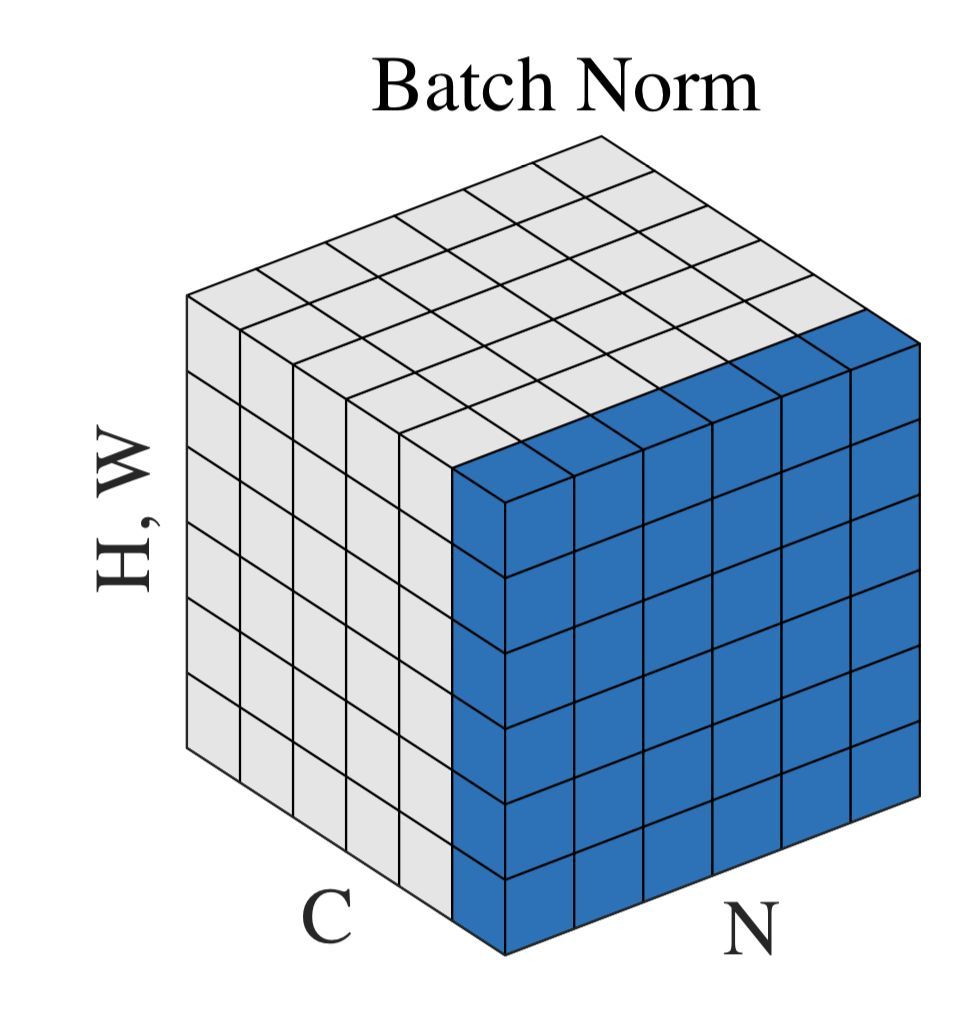
\includegraphics[width=1\textwidth]{Images/batchNorm.png}
		\end{minipage}
	}
	\item {
		\textit{Differentiable-augmentation:} is a set of differentiable image transformations used to augment data during training. The
		transformations are applied to both real and generated images. It enables the gradients to be propagated trough the augmentation
		back to the generator, regularizes the discriminator without manipulating the target distribution and maintains the balance of training
		dynamics. There are three choices of transformation: Translation, CutOut and Color.\\\\
		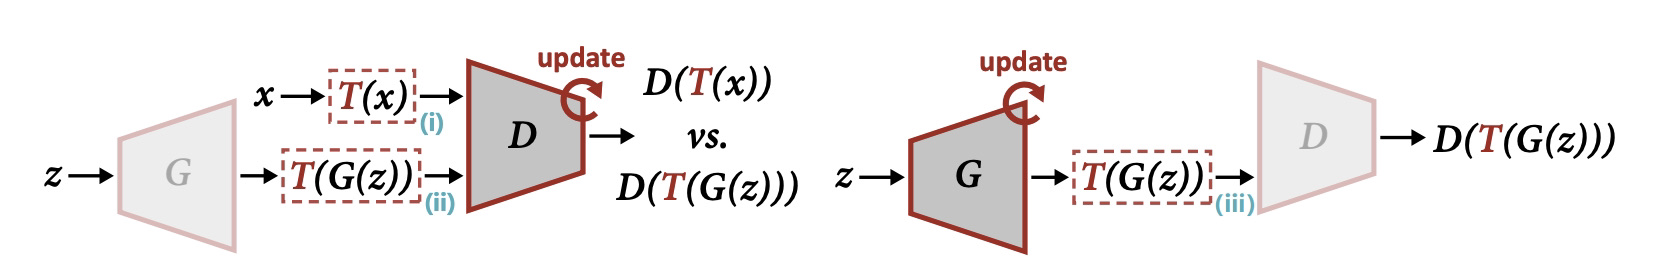
\includegraphics[width=0.9\textwidth]{Images/diffAugment.png}
	}
	\item {
		\begin{minipage}[t]{0.5\textwidth}
			\textit{ADAM optimization on G:} ADAM is a replacement optimization algorithm for stochastic gradient descent for training deep learning
			models; it combines the best properties of AdaGrad and RMSprop algorithms, to provide an optimization algorithm that can handle
			sparse gradients on noisy problems.\\
			In other words, ADAM can be looked at as a combination of both RMSprop and Stochastic Gradient Descent (SGD) with momentum: it uses
			the squared gradients to scale the learning rate like RMSprop and it takes advantage of momentum by using moving average of the gradient
			instead of gradient itself like SGD with momentum. \\
		\end{minipage}
		\hspace{0.02\linewidth}
		\begin{minipage}[t]{0.4\textwidth} 
			\vspace{-0.5cm}
			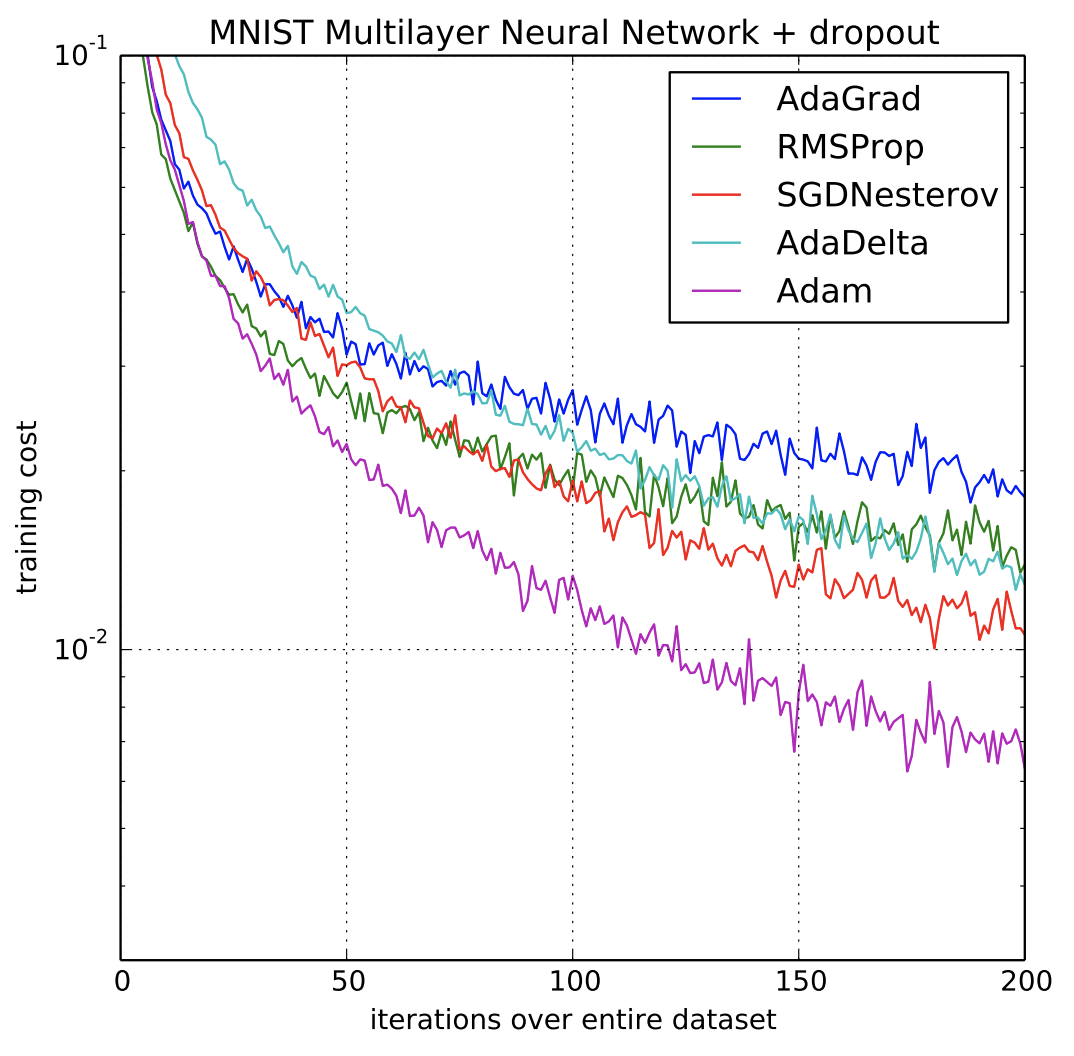
\includegraphics[width=1\textwidth]{Images/Adam.png}
		\end{minipage}	
	}
	\item {
		\begin{minipage}[t]{0.5\textwidth}
			\textit{GLU instead of ReLU in G:} Gated Linear Unit computes $GLU(a,b) = a \otimes \sigma(b)$, where $b$ is the gate that controls
			what information from $a$ is passed up to the following layer. This gating mechanism allows selection of features that are important
			for predicting the next feature; it also provides a mechanism to learn and pass along just the relevant info.
		\end{minipage}
		\hspace{0.02\linewidth}
		\begin{minipage}[t]{0.4\textwidth} 
			\vspace{-0.5cm}
			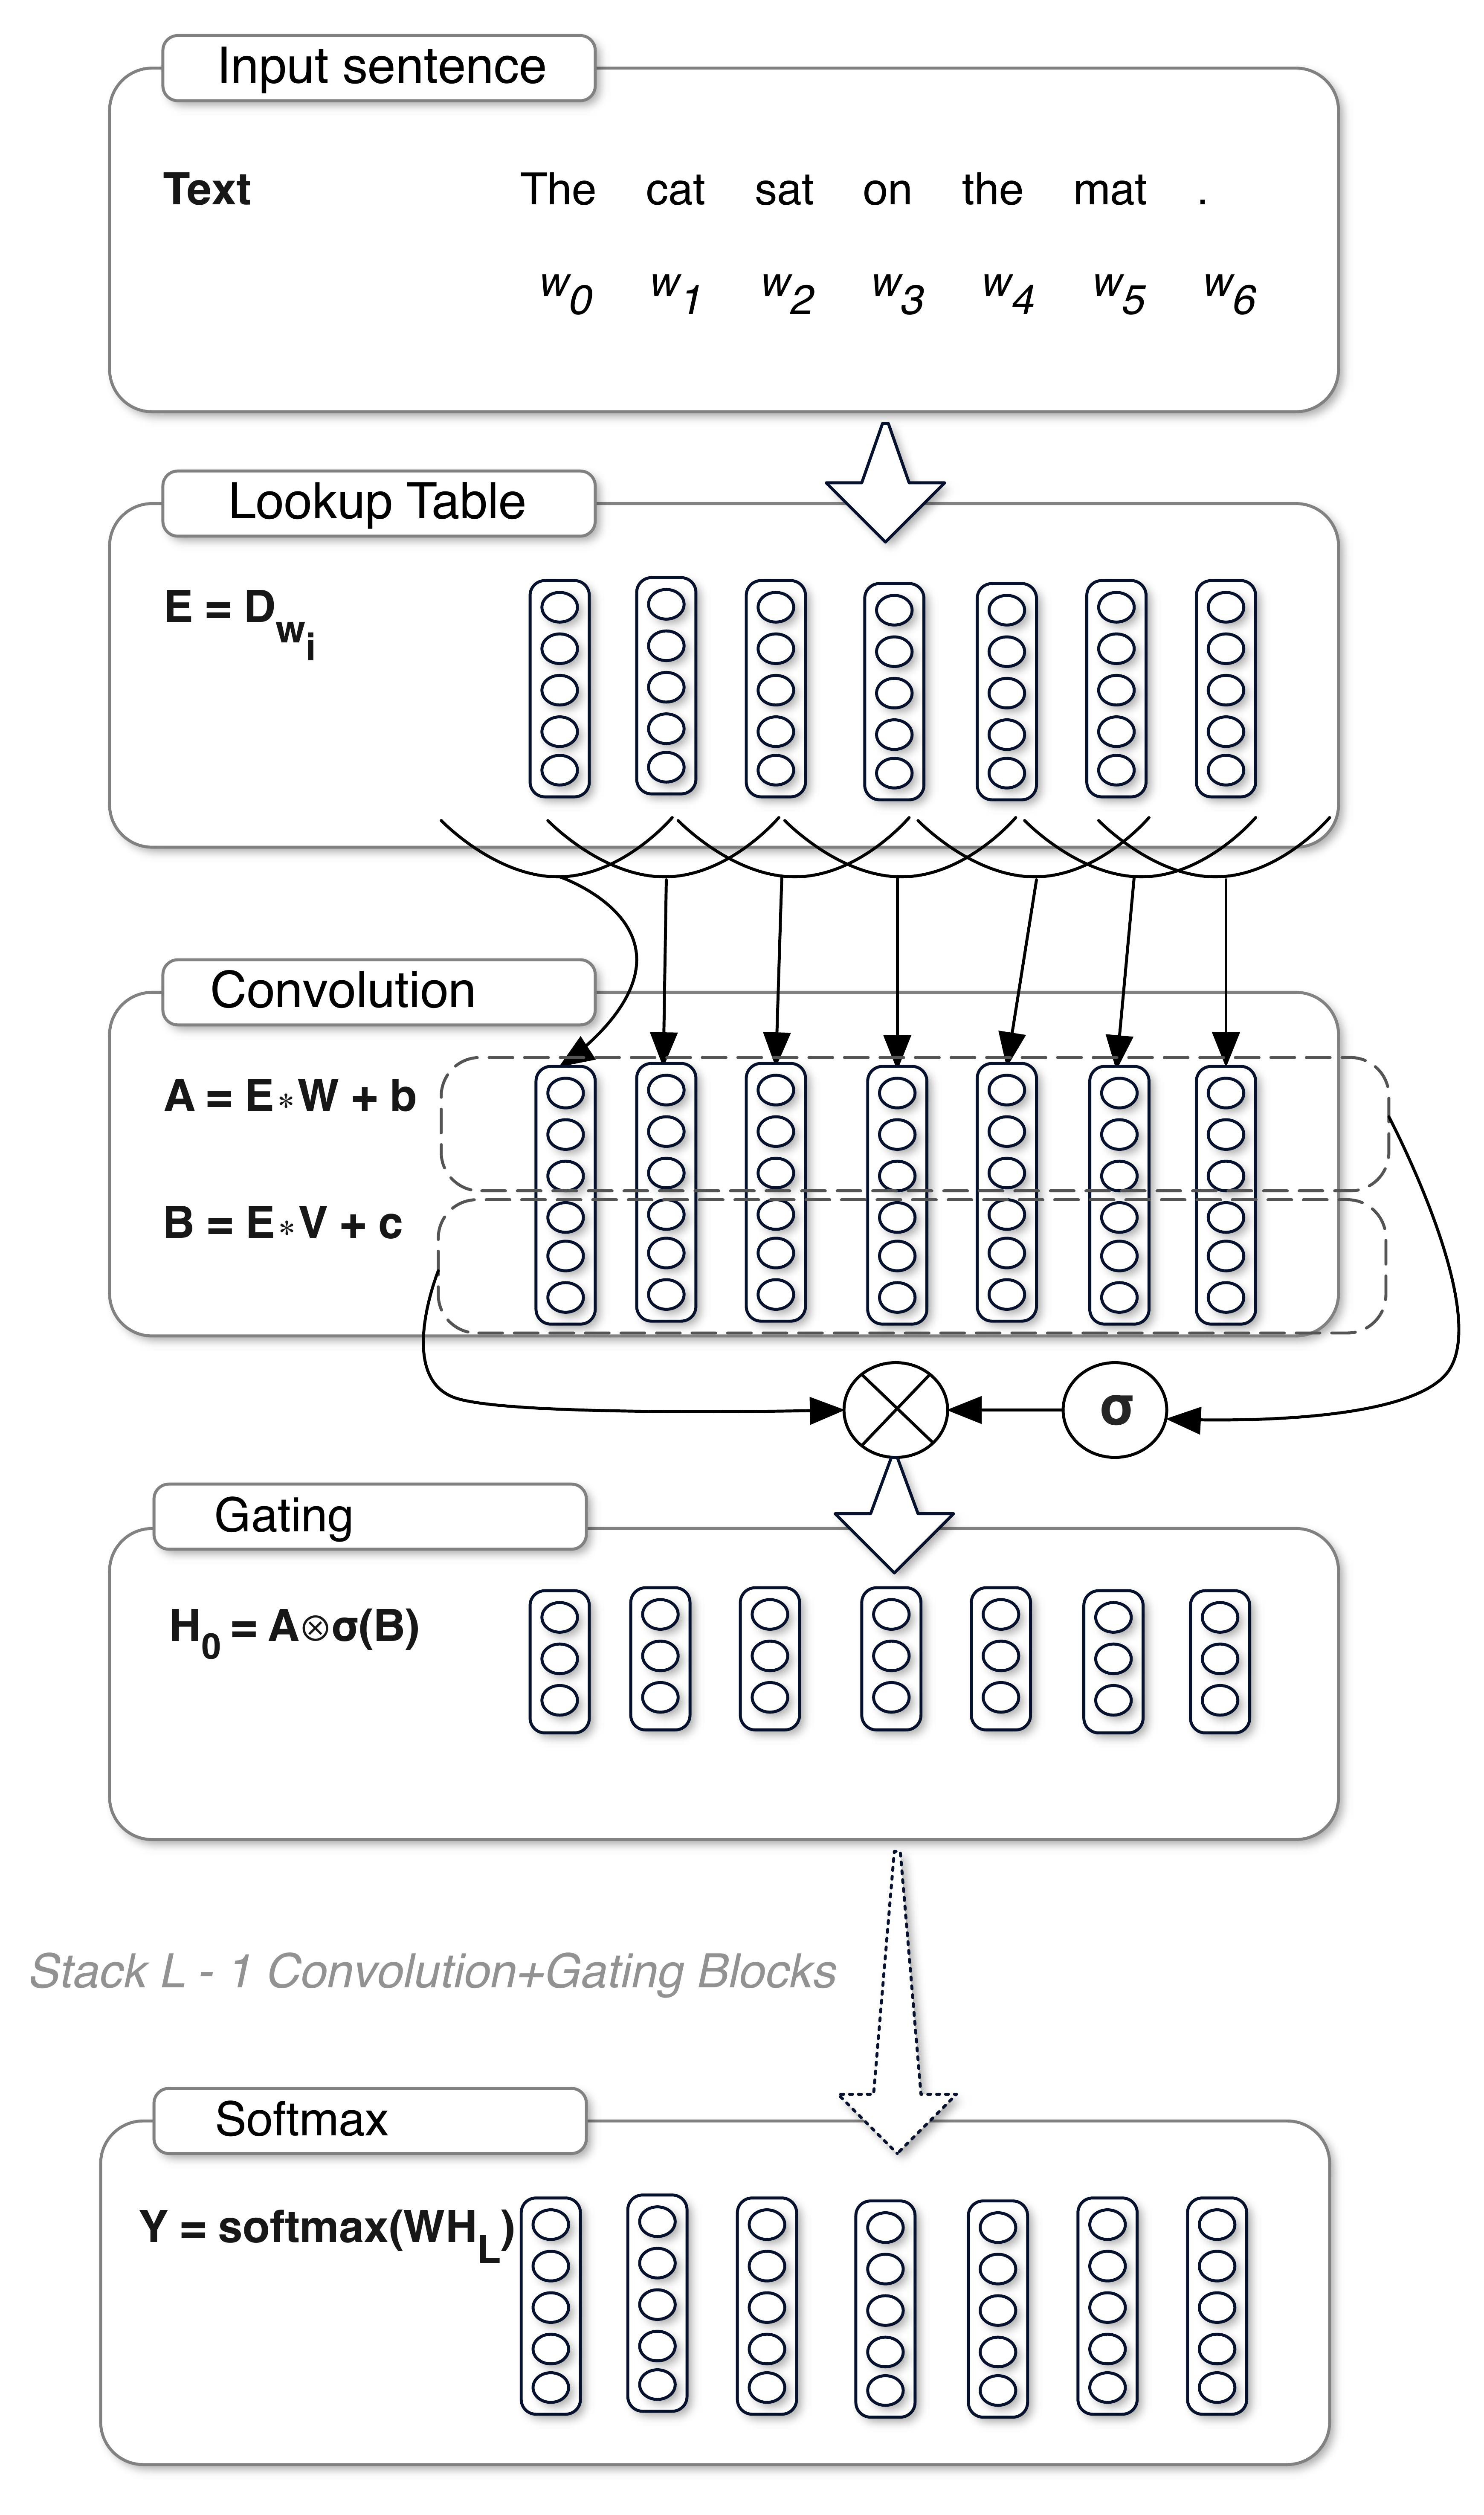
\includegraphics[width=1\textwidth]{Images/GLU.png}
		\end{minipage}
	}
\end{itemize} 



% IMPLEMENTATION CHOICES -------------------------------------------------------------------------

\section{Implementation and metrics choices}
\large

\subsection{Implementation}

Traditional GANs always required a lot of computational power in order to obtain good results.\\
Conversely, FastGAN has the big advantage of obtaining good results in a reasonable time also on non server-level hardware.
In fact we got decent results on NVIDIA GeForce RTX 2070 SUPER and, specially, on NVIDIA GeForce GTX 1050-Ti, 
respectively equipped with 8GB and 4GB of VRAM. More specifically we were able to train the GAN for 1000/2000 epochs: for each dataset this
took between $\sim$5hrs and $\sim$14hrs on the 2070 SUPER, and $\sim$2 days on the 1050-Ti. Those are very good results because, with the traditional
GANs, mostly on the 1050-Ti, probably it would have been impossible even just letting the train start.\\\\
Regarding the code implementation, while the original paper proposed a PyTorch version, we decided to reimplement it using 
TensorFlow.\\\\
Since the training needed a lot of time to execute, we used a checkpoint approach: in this way 
we were able to save the training status and resume the training whenever we wanted. 
More specifically we saved the current epoch number and the current weights of both the generator and
the discriminator.\\\\
Finally, we decided to generate output images in a grid format, in order to show more of them at the same time.


\subsubsection{Requirements}
\large

\begin{itemize}
	\item Python 3.8.x
	\item TensorFlow 2.x
	\item NVIDIA CUDA 11
	\item NVIDIA cuDNN 8
\end{itemize}
The above requirements are only the basic ones; in order to replicate the environment that we used, we have created
the "environment.yml" file that includes all the packages needed.
We were able to execute the project both on Windows and MacOS, but we ran the training only on Windows, 
in order to exploit the performance boost given by the CUDA hardware.


\subsection{Metrics}

Differently from the original paper, we used only Fréchet Inception Distance (FID) which
is a metric that calculates the distance between feature vectors calculated for real and 
generated images.
The score summarizes how similar the two groups are in terms of statistics on computer vision 
features of the raw images. Lower scores indicate the two groups of images are more similar, 
or have more similar statistics, with a perfect score being 0.0 indicating that the two 
groups of images are identical. The FID score is used to evaluate the quality of images 
generated by generative adversarial networks, and lower scores have been shown to correlate 
well with higher quality images. 
More specifically we calculated FID during training for each epoch, and we used it in order to
save model's weights only when it got better (lower) with respect to the previous best saved FID score:
this helps in maintaining high performances. 


% DATASET -------------------------------------------------------------------------	

\section{Dataset}
\large
The authors of the original paper used multiple datasets on both $256 \times 256$ and $1024 \times 1024$ resolutions. More specifically
they used: Animal-Face Dog and Cat, 100-Shot-Obama, Panda, Grumpy-cat, Flickr-Face-HQ, 
Oxford-flowers, Art paintings from WikiArt, Photographs on natural landscape from Unsplash, 
Pokemon, Anime face, Skull, Shell.\\\\ 
Since our hardware was not powerfull enough to do the training on photos with a resolution of $1024 \times 1024$, we decided to use only
datasets of resolution $256 \times 256$, and, more in details, we used the following datasets: 
\begin{itemize}
	\item Panda
	\item Obama
	\item Animal-Face Dog
	\item Animal-Face Cat
	\item Grumpy-cat\\
\end{itemize}
\begin{minipage}[t]{0.2\textwidth}
	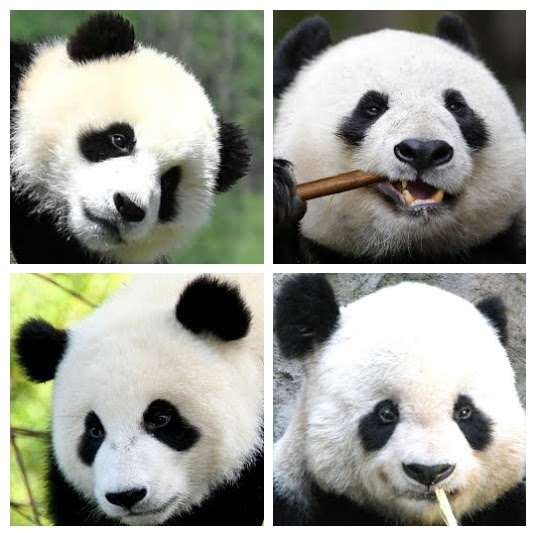
\includegraphics[width=1\textwidth]{Images/panda.jpg}
\end{minipage}
\begin{minipage}[t]{0.2\textwidth} 
	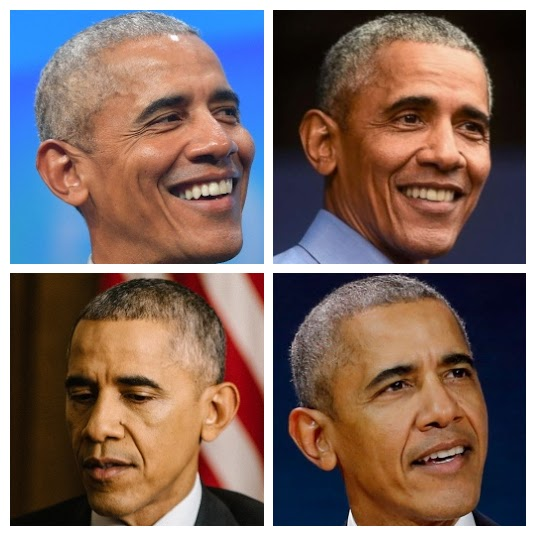
\includegraphics[width=1\textwidth]{Images/obama.jpg}
\end{minipage}
\begin{minipage}[t]{0.2\textwidth} 
	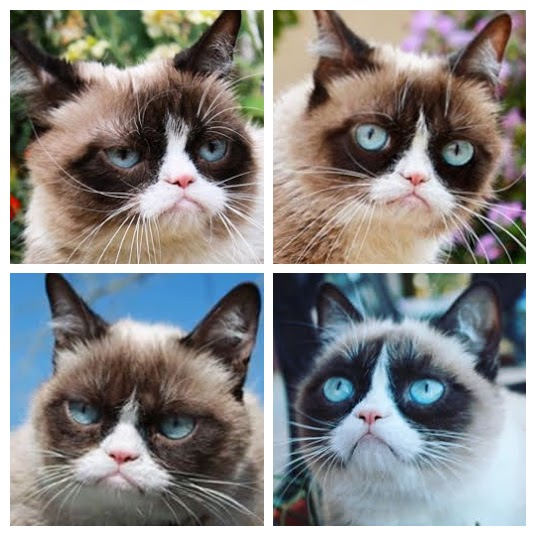
\includegraphics[width=1\textwidth]{Images/grumpy.jpg}
\end{minipage}
\begin{minipage}[t]{0.2\textwidth} 
	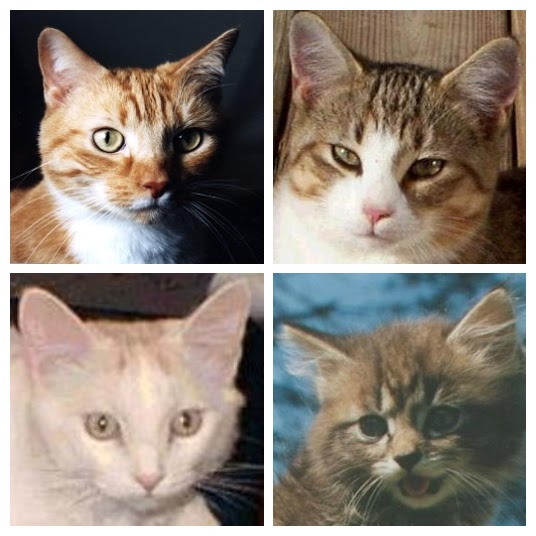
\includegraphics[width=1\textwidth]{Images/cat.jpg}
\end{minipage}
\begin{minipage}[t]{0.2\textwidth} 
	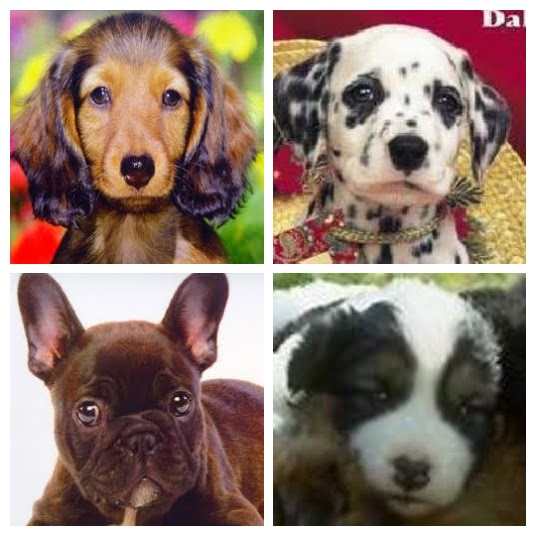
\includegraphics[width=1\textwidth]{Images/dog.jpg}
\end{minipage}

% EXPERIMENTS -------------------------------------------------------------------------

\section{Experiments}
\large
Here we show our experiments done on the datasets described in the previous section on two different
GPUs: NVIDIA GeForce RTX 2070 SUPER and NVIDIA GeForce GTX 1050-Ti. All the involved datasets consist 
of few images, where all of them have a resolution of 256$\times$256.\\\\
Regarding training times and output images:
\begin{itemize}
	\item {			 
		\textbf{\textit{Panda dataset:}} $\sim$4.5hrs for 1000 epochs on the 2070 SUPER
		\begin{figure}[H]
			\centering
			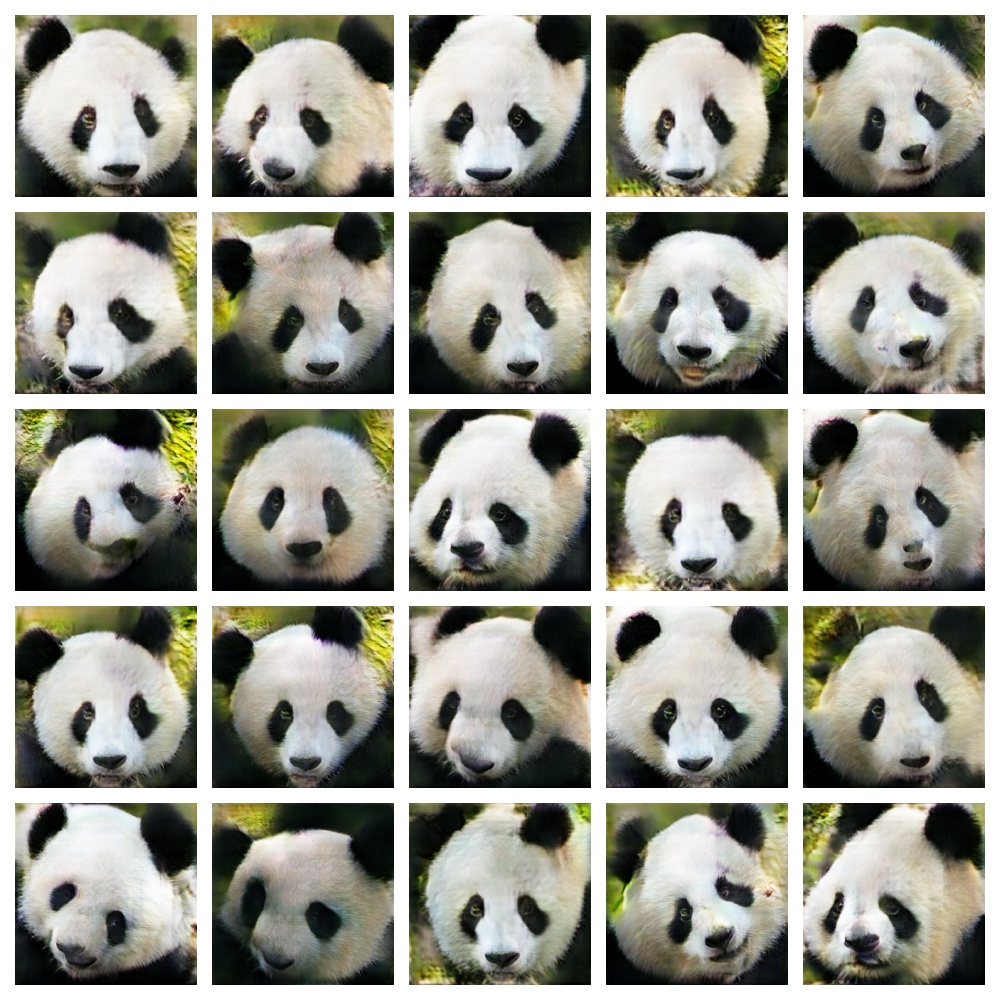
\includegraphics[width=0.5\textwidth]{Images/panda_exp.jpg}
		\end{figure}
	}
	\item {
		\textbf{\textit{Dogs dataset:}} $\sim$13.5hrs for 1400 epochs on the 2070 SUPER
		\begin{figure}[H]
			\centering
			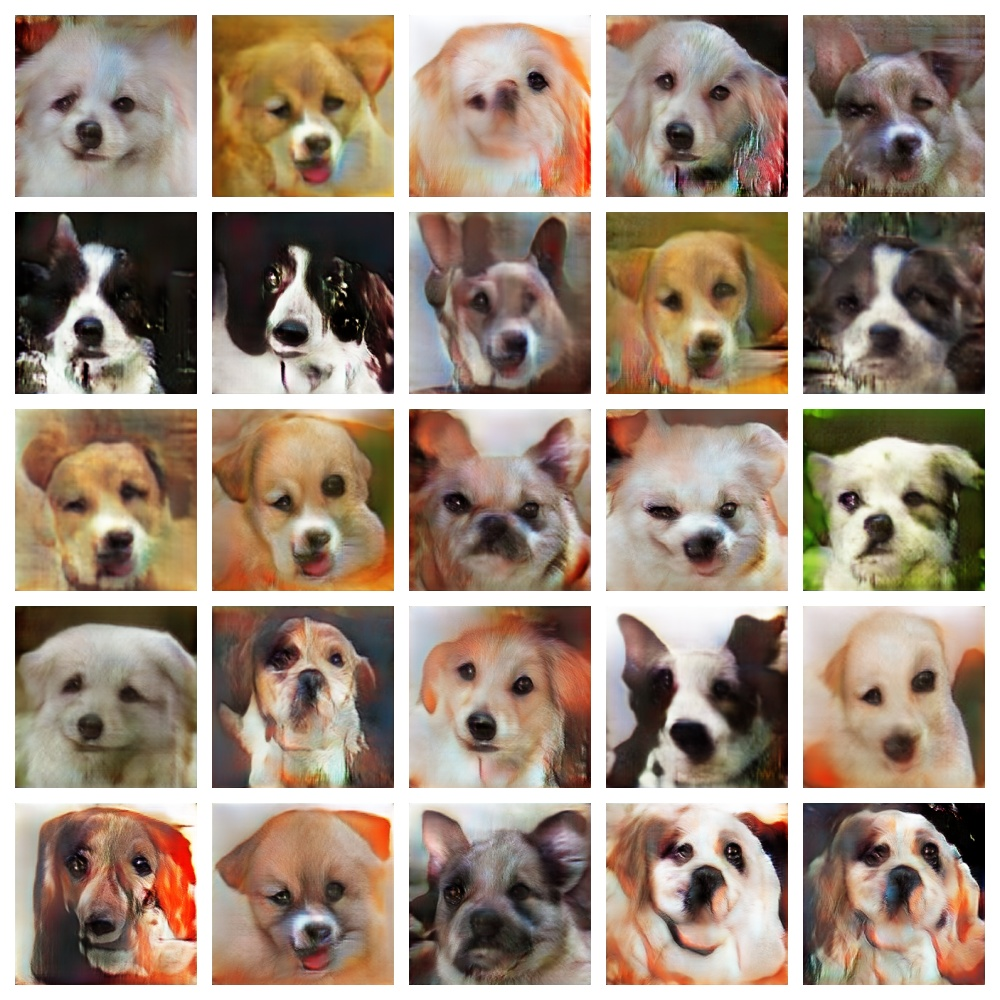
\includegraphics[width=0.5\textwidth]{Images/dogs_exp.jpg}
		\end{figure}
	}
	\item {
		\textbf{\textit{Obama dataset:}} $\sim$7hrs for 1700 epochs on the 2070 SUPER
		\begin{figure}[H]
			\centering
			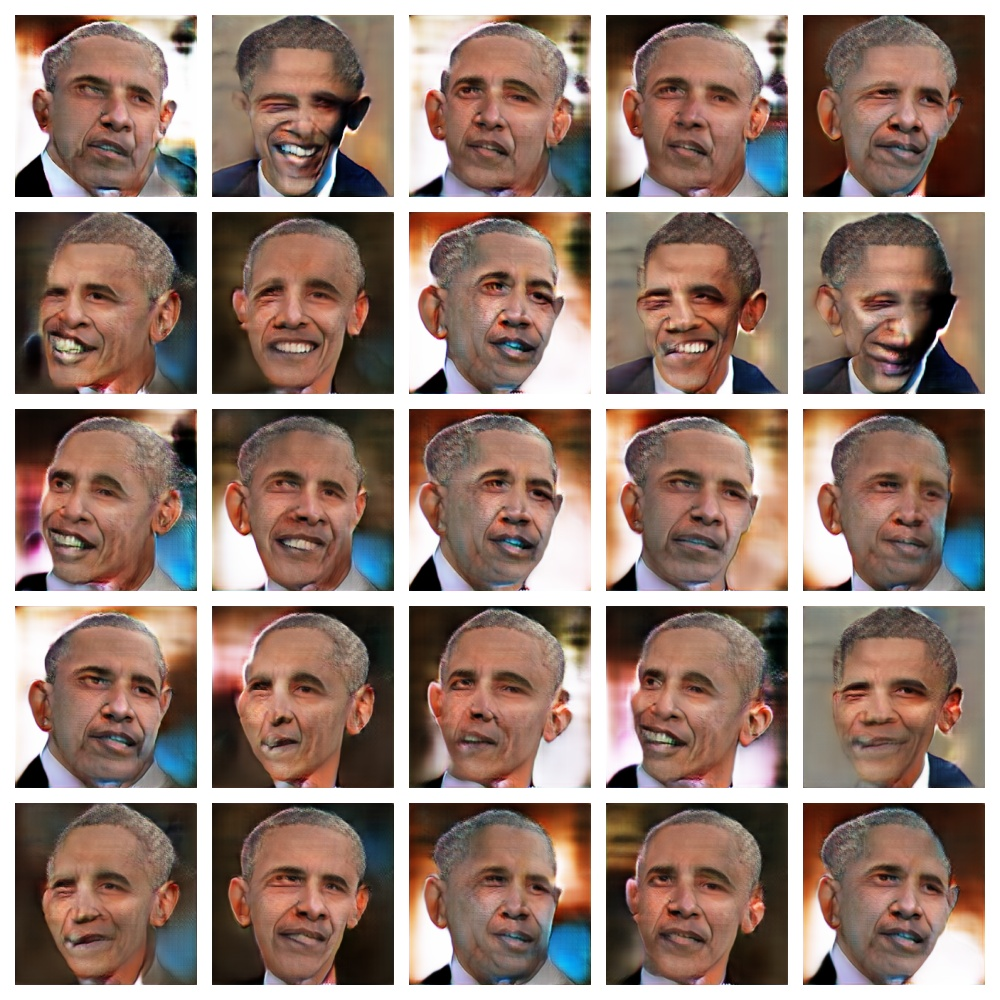
\includegraphics[width=0.5\textwidth]{Images/obama_exp.jpg}
		\end{figure}
	}
	\item {
		\textbf{\textit{Grumpy-cat dataset:}} $\sim$4.5hrs for 1000 epochs on the 2070 SUPER
		\begin{figure}[H]
			\centering
			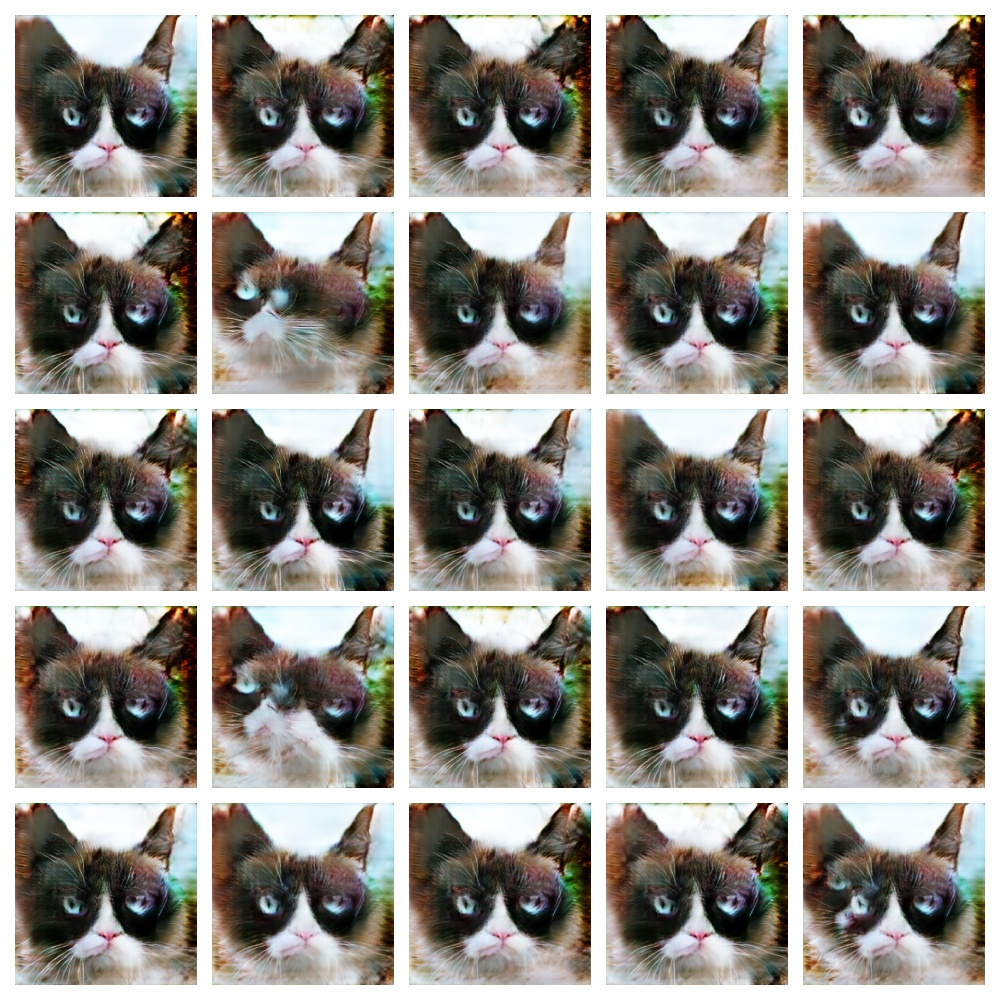
\includegraphics[width=0.5\textwidth]{Images/grumpy_exp.jpg}
		\end{figure}
	}
	\vspace*{4cm}
	\item {
		\textbf{\textit{Cats dataset:}} $\sim$45hrs for 1800 epochs on the 1050-Ti
		\begin{figure}[H]
			\centering
			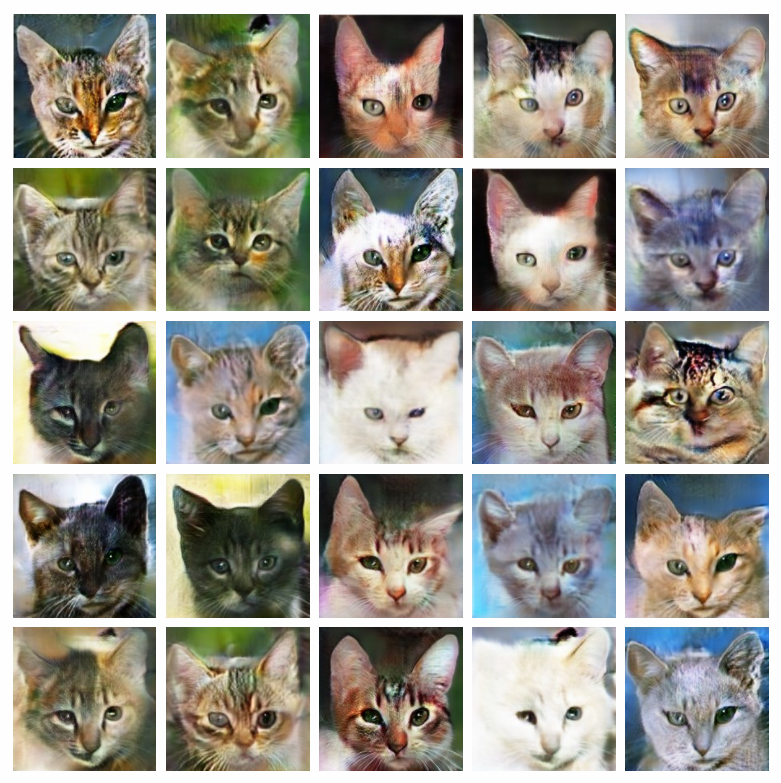
\includegraphics[width=0.5\textwidth]{Images/cats_exp.png}
		\end{figure}
	}
\end{itemize} 
As we can see in the above images and in the following table, thanks to FastGAN, we obtained
considerable results on small datasets and even on a 4GB 1050-Ti.\\
\begin{table}[H]
	\centering
	\footnotesize
	\begin{tabular}{ |M{3.4cm}|M{2.3cm}|M{2.3cm}|M{2.3cm}|M{2.3cm}|M{2.3cm}| }
		\cline{2-6}
		\multicolumn{1}{c|}{}&	
		\multicolumn{4}{c|}{\textbf{NVIDIA GeForce RTX 2070 SUPER}}&
		\multicolumn{1}{M{2.5cm}|}{\textbf{NVIDIA GeForce GTX 1050-Ti}}\\
		\hline
		\textbf{Dataset} 			&\textbf{Panda}			&\textbf{Dogs} 			&\textbf{Obama}			&\textbf{Grumpy Cat}		&\textbf{Cats}\\
		\hline
		\textbf{Number of images}   & 100 					& 389 					& 100 					& 100						& 159\\
		\textbf{Resolution}   		& 256$\times$256 		& 256$\times$256 		& 256$\times$256 		& 256$\times$256			& 256$\times$256\\
		\textbf{Batch size}			& 4						& 8 					& 8						& 8							& 4\\
		\textbf{Epochs} 			& 1000					& 1400 					& 1700 					& 1000						& 1800\\
		\textbf{Epoch Time} 		& $\sim$15s 			& $\sim$35s				& $\sim$15s				& $\sim$14s					& $\sim$103s\\
		\textbf{FID}				& $\sim$28				& $\sim$35				& $\sim$75				& $\sim$129					& $\sim$108\\						
		\hline
	\end{tabular}
	\newline\newline
	\caption{Training parameters and results on NVIDIA GeForce RTX 2070 SUPER and NVIDIA GeForce GTX 1050-Ti}
\end{table}

\subsection{Comparison with original paper's results}
\vspace*{-1.3cm}
\begin{center}
	\begin{minipage}[t]{0.48\textwidth} 
		\begin{figure}[H]
			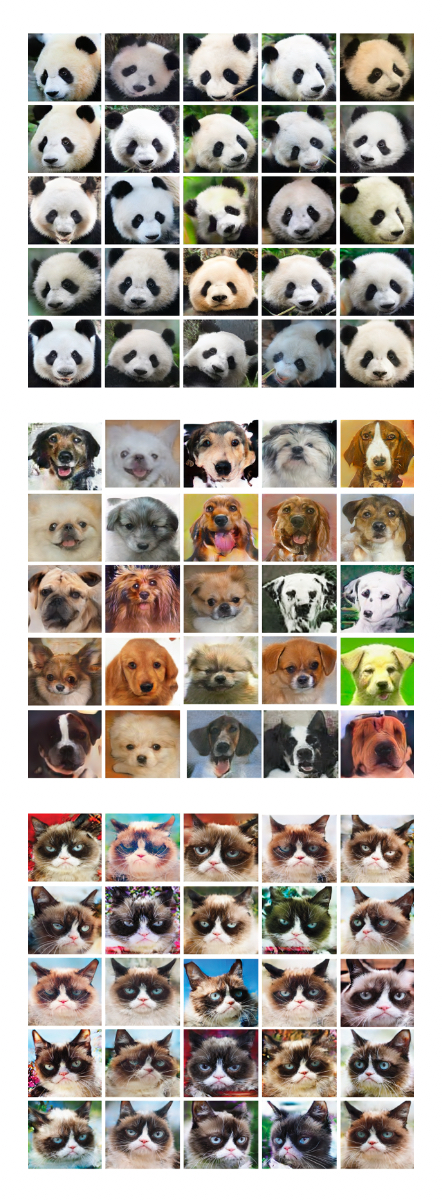
\includegraphics[width=1\textwidth]{Images/comparison.jpg}
			\caption{Original paper results}
		\end{figure}
	\end{minipage}
	\begin{minipage}[t]{0.48\textwidth} 
		\begin{figure}[H]
			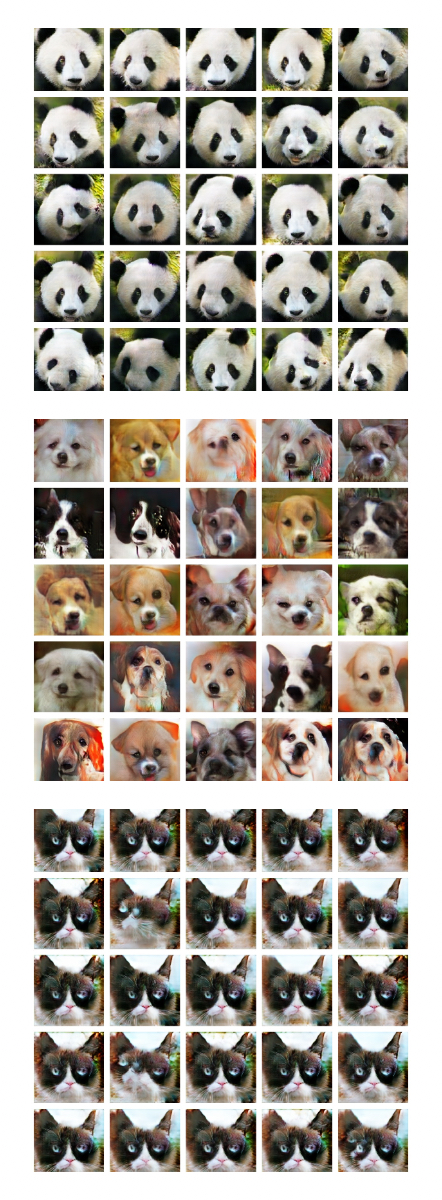
\includegraphics[width=1\textwidth]{Images/experiment.jpg}
			\caption{Our results}
		\end{figure}
	\end{minipage}
\end{center}
\begin{table}[H]
	\centering
	\footnotesize
	\begin{tabular}{ |M{2cm}M{2cm}M{2cm}M{2cm}M{2cm}M{2cm}M{2cm}| }
		\hline
			&		&\textbf{Panda}		&\textbf{Dogs} 		&\textbf{Obama}		&\textbf{Grumpy Cat}		&\textbf{Cats}			\\
		\hline
		\multicolumn{1}{|c}{}&	
		\multicolumn{1}{c|}{\textbf{Number of images}}&
		\multicolumn{1}{c}{100}&
		\multicolumn{1}{c}{389}&
		\multicolumn{1}{c}{100}&
		\multicolumn{1}{c}{100}&
		\multicolumn{1}{c|}{159}\\				
		\hline
		\multicolumn{1}{|M{2cm}|}{\textbf{FID on one RTX 2080-Ti}}&	
		\multicolumn{1}{c}{}&
		\multicolumn{1}{c}{10.03}&
		\multicolumn{1}{c}{50.66}&
		\multicolumn{1}{c}{41.05}&
		\multicolumn{1}{c}{26.65}&
		\multicolumn{1}{c|}{35.11}\\
		\hline
		\multicolumn{1}{|M{2cm}|}{\textbf{FID on one RTX 2070 SUPER}}&	
		\multicolumn{1}{c}{}&
		\multicolumn{1}{c}{$\sim$28}&
		\multicolumn{1}{c}{$\sim$35}&
		\multicolumn{1}{c}{$\sim$75}&
		\multicolumn{1}{c}{$\sim$129}&
		\multicolumn{1}{c|}{}\\
		\hline
		\multicolumn{1}{|M{2cm}|}{\textbf{FID on one GTX 1050-Ti}}&	
		\multicolumn{1}{c}{}&
		\multicolumn{1}{c}{}&
		\multicolumn{1}{c}{}&
		\multicolumn{1}{c}{}&
		\multicolumn{1}{c}{}&
		\multicolumn{1}{c|}{$\sim$108}\\
		\hline
	\end{tabular}
	\newline\newline
	\caption{FID score comparison between original paper (RTX 2080-Ti) and ours (NVIDIA GeForce RTX 2070 SUPER and NVIDIA GeForce GTX 1050-Ti)}
\end{table}

% CONCLUSION -------------------------------------------------------------------------

\section{Conclusion}
\large
As we discussed, given small datasets (sub-hundred images) and limited computing resources, GAN training can be stabilized
with an improved synthesis quality using skip-layer excitation mechanism (SLE) and self-supervised regularization on
the discriminator, which boost synthesis performance of the GAN.
Obviously, we obtained worse results with respect to the original paper, since we had more limited computing resources; said that,
we still got considerable results.

\end{document}
